
\documentclass[tikz, border=1mm]{standalone}

\usepackage{amsmath}

\usetikzlibrary{calc,angles,quotes}

\begin{document}
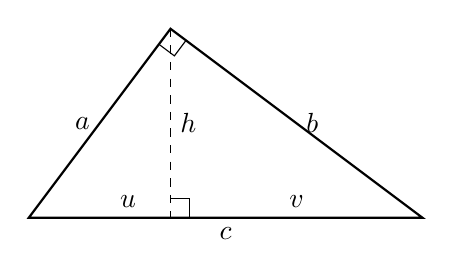
\begin{tikzpicture}[scale=1.0]

	% triangle 3 - 4 - 5
	\def\a{53.13}

	% points
	\coordinate (A) at (0,0);
	\coordinate (B) at ({3*cos(\a)},{3*sin(\a)});
	\coordinate (C) at (5,0);

	% feet of altitude from B to AC
	\coordinate (D) at ({3*cos(\a)},0);

	% triangle sides
	\draw[thick] (A) -- (B) -- (C) -- cycle;

	% altitude
	\draw[dashed] (B) -- (D);

	% right angle marker
	\pic [draw, angle radius=7pt, angle eccentricity=1]
	{right angle = A--B--C};
	\pic [draw, angle radius=7pt, angle eccentricity=1]
	{right angle = B--D--C};

	% side labels
	\node[left]  at ($(A)!0.5!(B)$) {$a$};
	\node[right] at ($(B)!0.5!(C)$) {$b$};
	\node[below] at ($(A)!0.5!(C)$) {$c$};

	% segment labels on altitude projection
	\node[above] at ($(A)!0.7!(D)$) {$u$};
	\node[above] at ($(D)!0.5!(C)$) {$v$};

	% height label
	\node[right] at ($(B)!0.5!(D)$) {$h$};

\end{tikzpicture}
\end{document}
